% Options for packages loaded elsewhere
\PassOptionsToPackage{unicode}{hyperref}
\PassOptionsToPackage{hyphens}{url}
%
\documentclass[
]{article}
\usepackage{amsmath,amssymb}
\usepackage{lmodern}
\usepackage{ifxetex,ifluatex}
\ifnum 0\ifxetex 1\fi\ifluatex 1\fi=0 % if pdftex
  \usepackage[T1]{fontenc}
  \usepackage[utf8]{inputenc}
  \usepackage{textcomp} % provide euro and other symbols
\else % if luatex or xetex
  \usepackage{unicode-math}
  \defaultfontfeatures{Scale=MatchLowercase}
  \defaultfontfeatures[\rmfamily]{Ligatures=TeX,Scale=1}
\fi
% Use upquote if available, for straight quotes in verbatim environments
\IfFileExists{upquote.sty}{\usepackage{upquote}}{}
\IfFileExists{microtype.sty}{% use microtype if available
  \usepackage[]{microtype}
  \UseMicrotypeSet[protrusion]{basicmath} % disable protrusion for tt fonts
}{}
\makeatletter
\@ifundefined{KOMAClassName}{% if non-KOMA class
  \IfFileExists{parskip.sty}{%
    \usepackage{parskip}
  }{% else
    \setlength{\parindent}{0pt}
    \setlength{\parskip}{6pt plus 2pt minus 1pt}}
}{% if KOMA class
  \KOMAoptions{parskip=half}}
\makeatother
\usepackage{xcolor}
\IfFileExists{xurl.sty}{\usepackage{xurl}}{} % add URL line breaks if available
\IfFileExists{bookmark.sty}{\usepackage{bookmark}}{\usepackage{hyperref}}
\hypersetup{
  pdftitle={REPORT: CUSTOMER BRAND PREFERENCES},
  pdfauthor={Ale F. Benages},
  hidelinks,
  pdfcreator={LaTeX via pandoc}}
\urlstyle{same} % disable monospaced font for URLs
\usepackage[margin=1in]{geometry}
\usepackage{graphicx}
\makeatletter
\def\maxwidth{\ifdim\Gin@nat@width>\linewidth\linewidth\else\Gin@nat@width\fi}
\def\maxheight{\ifdim\Gin@nat@height>\textheight\textheight\else\Gin@nat@height\fi}
\makeatother
% Scale images if necessary, so that they will not overflow the page
% margins by default, and it is still possible to overwrite the defaults
% using explicit options in \includegraphics[width, height, ...]{}
\setkeys{Gin}{width=\maxwidth,height=\maxheight,keepaspectratio}
% Set default figure placement to htbp
\makeatletter
\def\fps@figure{htbp}
\makeatother
\setlength{\emergencystretch}{3em} % prevent overfull lines
\providecommand{\tightlist}{%
  \setlength{\itemsep}{0pt}\setlength{\parskip}{0pt}}
\setcounter{secnumdepth}{-\maxdimen} % remove section numbering
\ifluatex
  \usepackage{selnolig}  % disable illegal ligatures
\fi

\title{REPORT: CUSTOMER BRAND PREFERENCES}
\author{Ale F. Benages}
\date{04/15/2021}

\begin{document}
\maketitle

\hypertarget{introduction}{%
\section{Introduction}\label{introduction}}

In this task I was required to analyze data from two different surveys,
one was complete and the other incomplete. The main difference, apart
from the length, was that the column containing the brand choices from
the incomplete survey contained a lot of useless information that had to
be discarded.

The main task was to use some machine learning models to learn about the
brand preference of customers. Then use this model to guess the brand
choice from the incomplete survey, and convert the useless survey into
something useful.

I was required to accomplish this task using R, and the machine learning
library: CARET.

\hypertarget{results}{%
\section{Results}\label{results}}

The constructed model was able to guess the brand choice from the
incomplete survey. It's impossible to define if the results are perfect
or not, because the ground truth was only available in the complete
dataset. But the similarity in the proportion of choices (plus the
similarity of the distribution of the selected features) was a very good
indicator that the model guessed accurately.

\hypertarget{brands-proportions}{%
\subsection{Brands Proportions}\label{brands-proportions}}

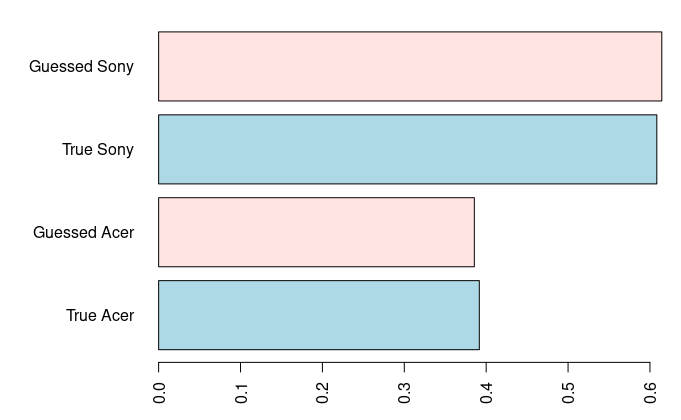
\includegraphics{/home/ale/Dropbox/UBIQUM/3.DAwithR/Task2:Classification.in.R/images/Proportions.png}

The exact values the graph are:

\begin{itemize}
\tightlist
\item
  Proportion of Guessed Sony: 0.61\\
\item
  Proportion of True Sony: 0.62\\
\item
  Proportion of Guessed Acer: 0.38\\
\item
  Proportion of True Acer: 0.39
\end{itemize}

\hypertarget{methods}{%
\section{Methods}\label{methods}}

\hypertarget{pipeline}{%
\subsection{Pipeline}\label{pipeline}}

The analysis suffered a lot of iterations, but the resulting report
reefers to the last one, and the general pipeline was divided in those
categories, each one including a lot of small steps:

1- \textbf{Dataset: Complete Survey}\\
Complete Survey \textgreater{} EDA + Pre-processing \textgreater{} Model
Training \textgreater{} Predictions \textgreater{} Feature Selection
\textgreater{} Predictions. 2- \textbf{Dataset: Incomplete Survey}\\
Incomplete Survey \textgreater{} EDA + Pre-processing.\\
3- \textbf{Features Comparison}\\
Then compared the selected features used to build the model with the
ones of the incomplete dataset.\\
4- \textbf{Guess Product Preference}\\
Used the model to guess the brand preference from the incomplete
dataset.\\
5- \textbf{Compare results with truth}\\
Compared the resulting \textbf{guessed proportion} of brand selection
with the \textbf{true proportion} of brand selection.

\hypertarget{dataset-complete-survey}{%
\subsection{1. Dataset: Complete Survey}\label{dataset-complete-survey}}

\hypertarget{eda}{%
\subsubsection{EDA}\label{eda}}

Started loading the \emph{CompleteResponses.csv}, and performing an EDA.
Graphs of each distribution can be founded on the original code.

\hypertarget{input-variables}{%
\subsubsection{Input Variables}\label{input-variables}}

\textbf{Numerical Variables} : Salary, Age, Credit\\
\textbf{Ordinal Categorical Variables} : Education Level\\
\textbf{Nominal Categorical Variables} : Zip Code, Car, Brand

\hypertarget{pre-processing}{%
\subsubsection{Pre-processing}\label{pre-processing}}

Some pre-processing tasks were required:\\
* \textbf{No missing values} were founded.\\
* \textbf{No Nan's} were founded.\\
* Adjusted some \textbf{datatypes}\\
* \textbf{Relabeling}, a 3rd file was attached, containing the
documentation of the codes used in the survey. I relabeled those codes
with legible labels.\\
* I applied \textbf{normalization} to the numerical variables, since
their scales were very different. After this step, all the affected
variables were scaled from 0 to 1. As this is a classification problem,
the scale of the features doesn't affect the output. This step is done
just to boost efficiency (improving accuracy and reducing computational
cost).

\hypertarget{model-training}{%
\subsubsection{Model Training}\label{model-training}}

\begin{itemize}
\tightlist
\item
  The Train/Test split, was done using caret::createDataPartition() in a
  proportion of 75/25\%.
\item
  Brand was defined as the output variable.
\end{itemize}

\hypertarget{models}{%
\paragraph{Models}\label{models}}

6 classification algorithms were trained using the training split of the
dataset:\\
- 2 different versions of Gradient Boosting Machine,\\
- 3 different versions of Random Forest Classification and\\
- 1 C5.0

\hypertarget{predictions-v0.1}{%
\subsubsection{Predictions (V0.1)}\label{predictions-v0.1}}

After training, the test split was used to make predictions with unseen
data. All the models selected performed well, but \textbf{the best was a
Random Forest Classifier, with an accuracy of 92,96\%.}

\hypertarget{feature-selection}{%
\subsubsection{Feature Selection}\label{feature-selection}}

Something known but not less important, is that running the models,
using the dataset with all the given features, requires a \textbf{lot}
of computational resources and time. Running the first iteration of the
6 models lasted approx. 4-6 hours. That's why after running each model,
the caret::varImp() function was included. This function evaluates the
\emph{importance} of each feature for each particular model, and assigns
them a score from 0 to 100.

This is the result of the selected model:
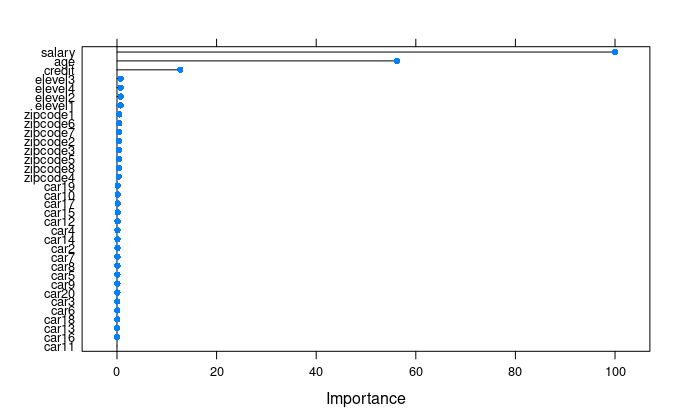
\includegraphics{/home/ale/Dropbox/UBIQUM/3.DAwithR/Task2:Classification.in.R/images/varImp.png}

The result is that the dataset can be reduced to just 3 meaningful
features: Salary, Age and Credit (the three numerical ones).

\hypertarget{predictions-reloaded}{%
\subsubsection{Predictions (reloaded)}\label{predictions-reloaded}}

After dropping most of the dataset's columns, I wanted to check
\emph{how much impact} this action had over the accuracy prediction. So
I repeated all the process (train/test split \textgreater{} training
\textgreater{} and predicting) with the new lighter dataset. The result
was a considerable diminution of processing time, from almost an hour
per model to approx a minute; with a minimal cost of reducing the
accuracy to 91,51\% (a difference of -0,015\%).

\textbf{Conclusion: I'm 95\% confident that the model classified the
customers preference in the complete survey with an accuracy from 0.9034
to 0.9258.}

\hypertarget{dataset-incomplete-survey}{%
\subsection{2. Dataset: Incomplete
Survey}\label{dataset-incomplete-survey}}

This step used the \emph{SurveyIncomplete.csv} and repeat most of the
EDA and pre-processing steps of the Complete Survey dataset.

Something important to mention is that the pre-processing tasks included
dropping all the unused input features \emph{(elevel, zipcode, car)}. AS
mentioned before, the output variable, brand, that contained a lot of
meaningless data was removed. The result was (again) a dataset with just
3 features: Salary, Age and Credit.

\hypertarget{features-comparison}{%
\subsection{3. Features' Comparison}\label{features-comparison}}

As any extra information of how the surveys were made was available nor
any complementary documentation, before using the reduced dataset from
the Incomplete Survey to perform predictions, was mandatory to check if
the distribution of each feature's samples between both surveys were
similar.

Fortunately their were \textbf{very similar!}, and this will be shown in
the next plots.

\hypertarget{salary-distribution}{%
\subsubsection{Salary Distribution}\label{salary-distribution}}

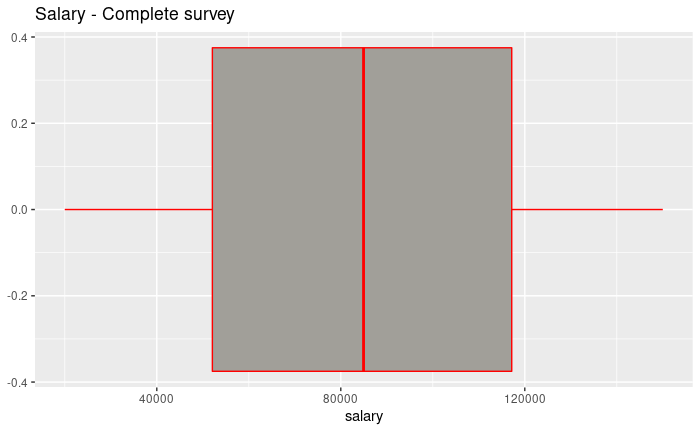
\includegraphics{/home/ale/Dropbox/UBIQUM/3.DAwithR/Task2:Classification.in.R/images/SalaryC.png}
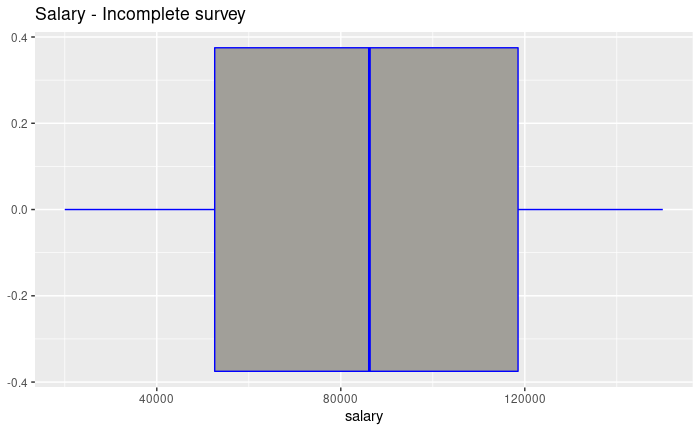
\includegraphics{/home/ale/Dropbox/UBIQUM/3.DAwithR/Task2:Classification.in.R/images/SalaryI.png}

\hypertarget{age-distribution}{%
\subsubsection{Age Distribution}\label{age-distribution}}

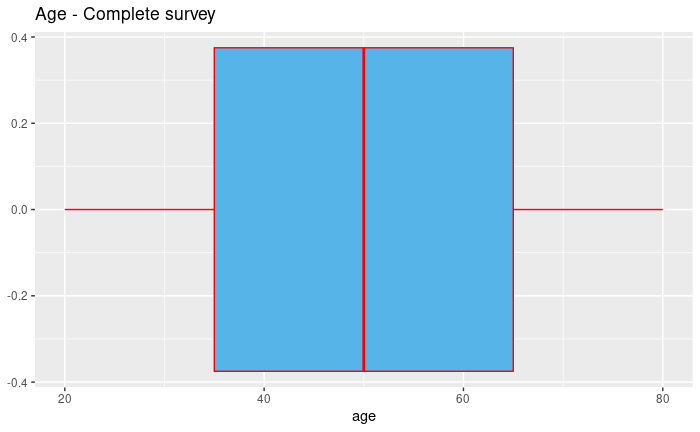
\includegraphics{/home/ale/Dropbox/UBIQUM/3.DAwithR/Task2:Classification.in.R/images/AgeC.png}
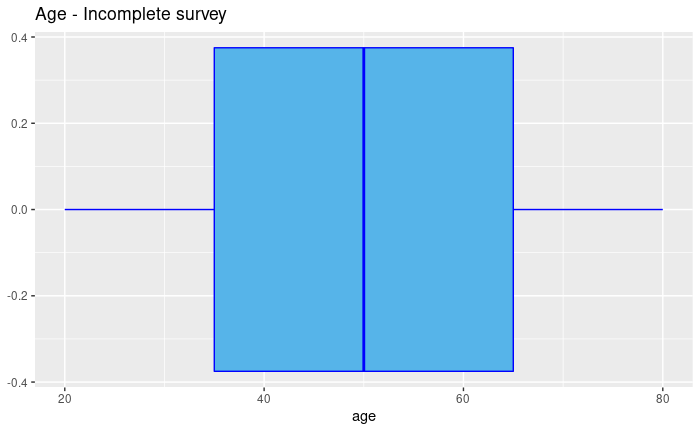
\includegraphics{/home/ale/Dropbox/UBIQUM/3.DAwithR/Task2:Classification.in.R/images/AgeI.png}

\hypertarget{credit-distribution}{%
\subsubsection{Credit Distribution}\label{credit-distribution}}

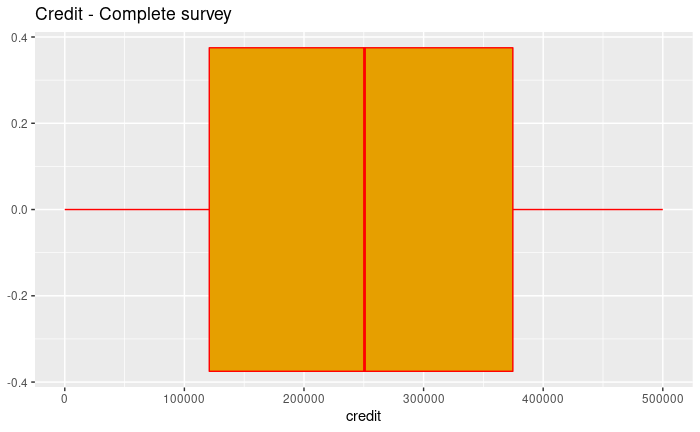
\includegraphics{/home/ale/Dropbox/UBIQUM/3.DAwithR/Task2:Classification.in.R/images/CrediC.png}
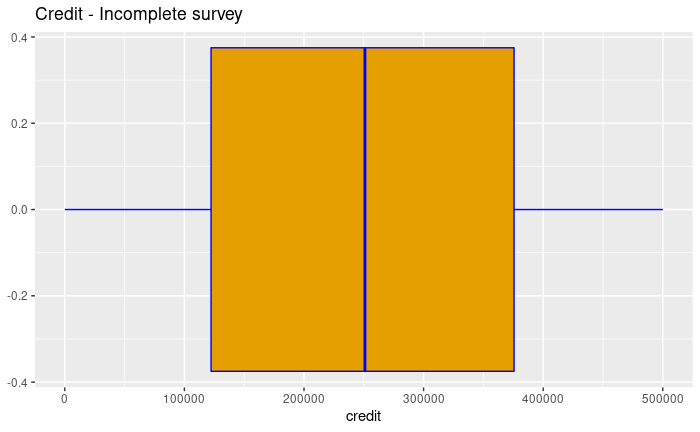
\includegraphics{/home/ale/Dropbox/UBIQUM/3.DAwithR/Task2:Classification.in.R/images/CredI.png}

\hypertarget{guess-product-preference}{%
\subsection{4. Guess Product
Preference}\label{guess-product-preference}}

\hypertarget{traintest-split.}{%
\subsubsection{Train/Test Split.}\label{traintest-split.}}

The brand choice was always my target variable, but in the
\emph{Incomplete Survey} this column has useless data and then was
removed. It was worthless to do the train/test split. In this case the
entire dataset was used to make predictions. It has no sense to separate
some data to test the accuracy of those predictions, since nobody knows
the exact answers (the ground truth is only in the Complete Survey
dataset).

\hypertarget{guessing}{%
\subsubsection{Guessing}\label{guessing}}

The Random Forest model was used to guess the brand choice of the
incomplete survey.
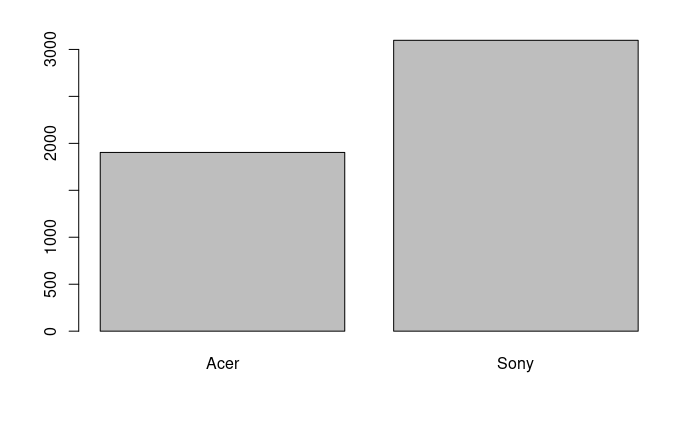
\includegraphics{/home/ale/Dropbox/UBIQUM/3.DAwithR/Task2:Classification.in.R/images/guess.png}

\hypertarget{conclusion}{%
\section{Conclusion:}\label{conclusion}}

I used labeled data to train a model. I got great values of accuracy in
my model and then I used this model to make guesses. Nobody knows the
correct answer, they are guesses based on the trained model, and it's
accuracy depends on the similarity of both populations. It's like a
model trained to predict fraud in online purchases, nobody knows in
advance what the client will do. But I can train some predictive models
with known past history, and based on some specific behaviors an alarm
can be raised to be on guard. Another example are the self driving cars:
their models can be trained to detect traffic lights, other cars,
cyclists, etc. but when the model is loaded and the car is moving it's
impossible to confirm everything the car will detect\ldots{} we must
build strong algorithms and believe in their guesses, that's why it's an
extremely complex problem.

\end{document}
